\documentclass[a4paper,12pt]{article}
\usepackage{graphicx}
\usepackage{hyperref}   % use for hypertext links, including those to external documents and URLs

\begin{document}



\begin{center}
\begin{Huge}
\textbf{{\LARGE Unit Test Visualisation\linebreak Unit test coding convention guide }}
\linebreak
\linebreak
\linebreak
\linebreak
\end{Huge}\end{center}




\begin{small}
\begin{flushleft}
\textbf{Author:} Keagan Phillips
\\
\textbf{Team:} Group 4
\\
\textbf{Course:} ELEN7046 - Software Technologies and Techniques
\\
\textbf{Date Submitted:} 25 June 2012
\\
\textbf{Source \& Documentation:} https://github.com/KeaganPhillips/Wit-Group-4-project/tree/master/Documentation
\linebreak
\linebreak
\linebreak
\linebreak
\linebreak
\end{flushleft}

\end{small}


\begin{flushleft}
\textbf{{\large Abstract}}
\end{flushleft}
This document describes the coding convention developers need to adhere to that enable the 'Unit Test Visualisation' system to extract test metadata. 
\clearpage


\tableofcontents


\clearpage

\section{Introduction}
\subsection{Overview}
The Unit Test Visualisation project extracts unit test metadata and present that data to the user on an HTML web front end as well as a PDF document. In order to extract the unit test metadata, developers must conform to a strict unit test coding standard. This convention is important because it provides the system to with an predictable, predefined framework from which unit test metadata can be extracted.
\subsection{Document Scope}
The rest of this document outlines this convention and discusses the technical reasoning around it.
\subsection{Assumptions Made}
This document assumes that the developer will be using the 'Visual Studio Unit Testing Framework'\cite{testFramework} as a unit test testing framework, and that the developer is familiar with the product.

\section{Organising Tests}
\subsection{Folder structure}
Figure \ref{fig1} depicts the folder structure that tests should conform to. As depicted, all classes for which there are test written for should have their own folders and must be contained within the parent ClassesUnderTest folder. Each class folder (e.g. “Account”) in turn may contain one or more "Test" folders, as a class can have multiple tests. A test on the other hand may have one or more scenarios. The scenario source files is where the actual automated test code will be written.\\
\linebreak
This structure makes it very easy for developers to arrange, find and maintain unit tests.

\begin{center}
	\begin{figure}
		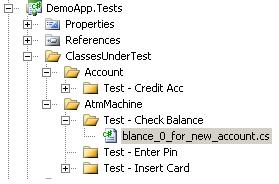
\includegraphics{solution_exlorer.JPG}
			\caption{}	
			\label{fig1}       
	\end{figure}	
\end{center}


\section{Test Scenarios}
\subsection{Given When Then}
Test scenarios are written using the 'Given / When / Then'\cite{gwt} convention. Each scenario must implement the IScenario interface. Figure \ref{fig2} shows a code snippet of this interface.
\subsection{IScenario Interface}
By implementing IScenario, developers are forced to explicitly provide 'Given' and 'When' descriptions for the test scenario in question, where 'Given' is an description of the initial context (initial state) of the class and it's dependencies and 'When' is an description of the event that occurs. Developer implement the ScenarioDescription property to provide a meaningful explanation of the test scenario. The ClassUnderTest property returns the class type for which the scenario is applicable. \\
\linebreak
The IScenario interface also provides Given and When methods where developers implement the code that sets up the initial context (i.e. given) and execute the event (i.e. when).\\
\linebreak
The developer must decorate their test method with at 'Then' C\# attribute as shown in figure \ref{fig3} to provide a meaningful description of the expected state of the class and dependencies after the event occurred. The reason for using attributes in this case is because a test may have more than one test criteria 

\begin{center}
	\begin{figure}
		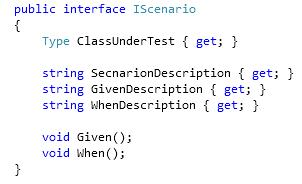
\includegraphics{IScenario.JPG}
			\caption{}	
			\label{fig2}       
	\end{figure}	
\end{center}

\begin{center}
	\begin{figure}
		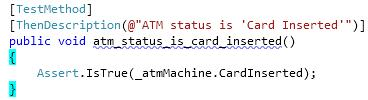
\includegraphics{ThenDesc.JPG}
			\caption{}	
			\label{fig3}       
	\end{figure}	
\end{center}

\subsection{The TestName Attribute}
Each scenario must be decorated with the TestName C\# Attribute as shown in Figure \ref{fig4}. The framework uses this attribute to determine the test the scenario belongs to.

\subsection{The TestHelper}
Each scenario must call 'TestHelper.SetupTest(this);' (see Figure \ref{fig4}) as part of the test setup. This helper method will call the IScenario.Given() and IScenario.When() methods for the current class to ensure the the initial context is setup and the event is fired.

\begin{center}
	\begin{figure}
		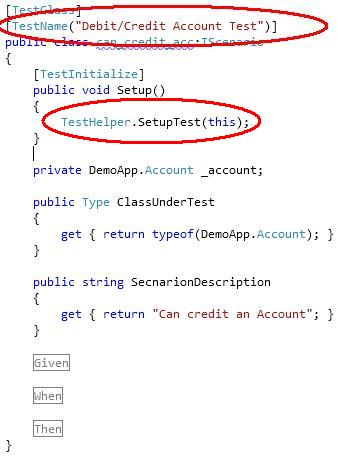
\includegraphics{TestNameAttribute.JPG}
			\caption{}	
			\label{fig4}       
	\end{figure}	
\end{center}


\section{Conclusion}
By following these conversions, the framework should extract the unit test metadata to be presented to the user on the front end.


\clearpage

\begin{thebibliography}{5}
\bibitem{gwt} Structure your test using Given/When/Then; Tested Objects 1.0 Users' Guide;  \url{http://testedobjects.sourceforge.net/m2-site/main/documentation/docbkx/html/user-guide/ch03s04.html}

\bibitem{attributes} \begin{flushleft}
Attributes (C\# Programming Guide); MSDN 
\end{flushleft}\url{http://msdn.microsoft.com/en-us/library/z0w1kczw%28v=vs.80%29.aspx}

\bibitem{testFramework} \begin{flushleft}
Visual Studio Unit Testing Framework; wikipedia
\end{flushleft} \url{http://en.wikipedia.org/wiki/Visual_Studio_Unit_Testing_Framework}

\end{thebibliography}

 


\end{document}